\title{A Very Simple \LaTeXe{} Template}
\author{Don Jones\\ \it{Temple University}}
\date{\today}

\documentclass[11pt]{article}
\usepackage{amsfonts,amssymb,amscd,amsthm,xspace}
\usepackage{graphicx}
\usepackage{lscape}

\usepackage{epstopdf}
\usepackage{booktabs}
\usepackage{rotating}
\usepackage{listings}
\usepackage{pdflscape}
\usepackage{amsmath}
\usepackage[section]{placeins}
\usepackage{feynmf}
\usepackage{caption}
\usepackage[usenames,dvipsnames]{xcolor}
\usepackage[square, numbers, comma, sort&compress]{natbib} % Use the natbib refe
\setlength{\parindent}{0pt}
\setlength{\parskip}{2.0ex plus0.5ex minus0.2ex}
\usepackage{vmargin}

\RequirePackage[utf8]{inputenc} % Allows the use of international characters (e.
\setmarginsrb   { 1.0in}  % left margin
                { 1.0in}  % top margin
                { 1.0in}  % right margin
                { 1.0in}  % bottom margin
                {  2pt}  % head height
                {0.25in}  % head sep
                {   59pt}  % foot height
                { 0.5in}  % foot sep
\title{Equations of Radioactive Decay of Isoptopes in a Decay Chain}


\begin{document}



\maketitle


\begin{abstract}
%% Text of abstract
In this document I show how to solve the coupled differential equations which describe the decay of isotopes in a decay chain. In this paper the initial condition is chosen as only the parent isotope existing at $t=0$. If a daughter isotope in a decay chain has a significantly shorter decay time constant than the parent it is possible to arrive at secular equilibrium where the decay rates of the daughter and parent isotopes are equal. For the more realistic case of approximate secular equilibrium I calculate the ratio of the parent to daughter decay rates (equilibrium constants). I show how this works specifically in the decay chain of $^{227}_{89}$Ac down to the stable isotope $^{207}_{82}$Pb. At equilibrium one would expect a total of 5 alphas for each Ac-227 decay, but one actually gets 5.015 alphas per Ac-227 decay. 
\end{abstract}


Keywords: half-life, decay chain, isotopes
%% keywords here, in the form: keyword \sep keyword

%% MSC codes here, in the form: \MSC code \sep code
%% or \MSC[2008] code \sep code (2000 is the default)



%%
%% Start line numbering here if you want
%%
%\linenumbers

%% main text
\section{Coupled Equations of a Decay Chain}
\label{S:1}
In scientific research radioactive isotopes are often utilized both as a source for calibrating instruments and as a subject of study themselves. It is desireable to know the equations governing the decay of a given set of isotopes. For a single isotope that has no parent isotopes in the material of interest, the number of atoms of that isotope is given by the simple and familiar decay equation:
\begin{equation}
\label{eq:parent_decay_rate}
\frac{dN(t)}{dt}=-\lambda N(t),
\end{equation} 
which has the simple solution 
\begin{equation}
\label{eq:N0}
N(t)=N(0)e^{-\lambda t}
\end{equation}
where $\lambda$ is the decay constant and $N(0)$ represents the number of atoms of the isotope at $t=0$. 

In a decay chain the number of atoms of each isotope depends on the rate of production of the parents as well as the rate of decay so that the rate of decay of each isotope depends upon the decay rate of all isotopes above it in the chain. This can described by the following set of coupled differential equations:
\begin{equation}
\label{eq:decay_chain}
\begin{array}{lcl}\dot{N}_0(t)&=&-\lambda_0N_0(t)\\
\dot{N}_1(t)&=&-\lambda_1N_1(t)+\lambda_0N_0(t)\\
~&\vdots&~\\
\dot{N}_n(t)&=&-\lambda_nN_n(t)+\lambda_{n-1}N_{n-1}(t)
\end{array}
\end{equation}
These equations can be solved in order using an integrating factor. An ODE of the form 
\begin{equation}
\label{eq:integrating_factor}
\frac{dy(t)}{dt}+p(t)y(t)=q(t),
\end{equation}
can be solved using the integrating factor $e^{\int^t p(t^{\prime})dt^{\prime}}$ giving the following solution:
\begin{equation}
\label{eq:ODE_solution}
y(t)=\frac{\int e^{\int^tp(t^{\prime})dt^{\prime}}q(t)dt + c}{e^{\int^tp(t^{\prime})dt^{\prime}}}.
\end{equation}
If we assume that at $t=0$ we start with only the parent isotope, Eq. \ref{eq:ODE_solution} together with Eq. \ref{eq:N0} yields
\[
N_1(t)=\lambda_0N_0(0)\left(\frac{e^{-\lambda_0t}-e^{-\lambda_1t}}{\lambda_1-\lambda_0}\right).
\]
Inserting this into the equation for $N_2(t)$ and solving similarly gives
\[
N_2(t)=\lambda_0\lambda_1N_0(0)\left(\frac{e^{-\lambda_0t}-e^{-\lambda_2t}}{(\lambda_1-\lambda_0)(\lambda_2-\lambda_0)}-\frac{e^{-\lambda_1t}-e^{-\lambda_2t}}{(\lambda_1-\lambda_0)(\lambda_2-\lambda_1)}\right).
\]
For $N_3(t)$ this gives
\begin{align}
\label{eq:N3}
N_3(t)=\lambda_0\lambda_1\lambda_2N_0(0)\left[\frac{e^{-\lambda_0t}-e^{-\lambda_3t}}{(\lambda_1-\lambda_0)(\lambda_2-\lambda_0)(\lambda_3-\lambda_0)}\right.&-\frac{e^{-\lambda_1t}-e^{-\lambda_3t}}{(\lambda_1-\lambda_0)(\lambda_2-\lambda_1)(\lambda_3-\lambda_1)}\notag\\-\frac{e^{-\lambda_2t}-e^{-\lambda_3t}}{(\lambda_1-\lambda_0)(\lambda_2-\lambda_0)(\lambda_3-\lambda_2)}&\left.+\frac{e^{-\lambda_2t}-e^{-\lambda_3t}}{(\lambda_1-\lambda_0)(\lambda_2-\lambda_1)(\lambda_3-\lambda_2)}\right].
\end{align}
For $N_4(t)$ this gives
\begin{align}
\label{eq:N4}
N_4(t)=\alpha\left[\frac{e^{-\lambda_0t}-e^{-\lambda_4t}}{(\lambda_1-\lambda_0)(\lambda_2-\lambda_0)(\lambda_3-\lambda_0)(\lambda_4-\lambda_0)}\right.&-\frac{e^{-\lambda_1t}-e^{-\lambda_4t}}{(\lambda_1-\lambda_0)(\lambda_2-\lambda_1)(\lambda_3-\lambda_1)(\lambda_4-\lambda_1)}\notag\\-\frac{e^{-\lambda_2t}-e^{-\lambda_4t}}{(\lambda_1-\lambda_0)(\lambda_2-\lambda_0)(\lambda_3-\lambda_2)(\lambda_4-\lambda_2)}&+\frac{e^{-\lambda_2t}-e^{-\lambda_4t}}{(\lambda_1-\lambda_0)(\lambda_2-\lambda_1)(\lambda_3-\lambda_2)(\lambda_4-\lambda_2)}\notag\\-\frac{e^{-\lambda_3t}-e^{-\lambda_4t}}{(\lambda_1-\lambda_0)(\lambda_2-\lambda_0)(\lambda_3-\lambda_0)(\lambda_4-\lambda_3)}&-\frac{e^{-\lambda_3t}-e^{-\lambda_4t}}{(\lambda_0-\lambda_1)(\lambda_2-\lambda_1)(\lambda_3-\lambda_1)(\lambda_4-\lambda_3)}\notag\\+\frac{e^{-\lambda_3t}-e^{-\lambda_4t}}{(\lambda_1-\lambda_0)(\lambda_2-\lambda_0)(\lambda_3-\lambda_2)(\lambda_4-\lambda_3)}&\left.-\frac{e^{-\lambda_3t}-e^{-\lambda_4t}}{(\lambda_1-\lambda_0)(\lambda_2-\lambda_1)(\lambda_3-\lambda_2)(\lambda_4-\lambda_3)}\right],
\end{align}
where $\alpha=\lambda_0\lambda_1\lambda_2\lambda_3N_0(0)$.
Each successive equation in the decay chain becomes more complicated with $2^{n-1}$ terms; however, often only one or a few terms dominate the expression as time progresses. Take for example the decay chain of $^{227}$Ac to $^{211}$Pb as follows:
\begin{equation}
\label{eq:decay_chain_diagram}
^{227}\text{Ac}\xrightarrow[t_{1/2}=21.8 y]{\alpha}~^{227}\text{Th}\xrightarrow[t_{1/2}=18.7 d]{\alpha}~^{223}\text{Ra}\xrightarrow[t_{1/2}=11.4 d]{\beta^-}~^{219}\text{Rn}\xrightarrow[t_{1/2}=3.96 s]{\alpha}~^{215}\text{Po}\xrightarrow[t_{1/2}=1.78ms]{\alpha}~^{211}\text{Pb}.
\end{equation}
Using $\lambda_0=\lambda_{Ac}=1.01\times10^{-9}$~s$^{-1}$, $\lambda_1=\lambda_{Th}=4.29\times10^{-7}$~s$^{-1}$, $\lambda_2=\lambda_{Ra}=7.02\times10^{-7}$~s$^{-1}$, and $\lambda_3=\lambda_{Rn}=0.175$~s$^{-1}$, we can approximate $N_3(t)$ as follows:
\begin{align}
N_3(t)&\approx\lambda_0\lambda_1\lambda_2N_0(0)\left[\frac{e^{-\lambda_0t}-e^{-\lambda_3t}}{\lambda_1\lambda_2\lambda_3}-\frac{e^{-\lambda_1t}-e^{-\lambda_3t}}{\lambda_1(\lambda_2-\lambda_1)\lambda_3}-\frac{e^{-\lambda_2t}-e^{-\lambda_3t}}{\lambda_1\lambda_2\lambda_3}-\frac{e^{-\lambda_2t}-e^{-\lambda_3t}}{\lambda_1(\lambda_2-\lambda_1)\lambda_3}\right]\\&=\frac{\lambda_0}{\lambda_3}N_0(0)\left[\left(e^{-\lambda_0t}-e^{-\lambda_2t}\right)-\frac{\lambda_2\left(e^{-\lambda_1t}+e^{-\lambda_2t}-2e^{-\lambda_3t}\right)}{(\lambda_2-\lambda_1)}\right]
\end{align}
With $\lambda_3=0.175$~s$^{-1}$, the last term involving $e^{-\lambda_3t}$ becomes negligible in less than a minute leaving
\begin{align}
\label{eq:N3approx1}
N_3(t)&\approx\frac{\lambda_0}{\lambda_3}N_0(0)\left[\left(e^{-\lambda_0t}-e^{-\lambda_2t}\right)-\frac{\lambda_2\left(e^{-\lambda_1t}+e^{-\lambda_2t}\right)}{(\lambda_2-\lambda_1)}\right]\notag\\&=\frac{t^{(3)}_{1/2}}{t^{(0)}_{1/2}}N_0(0)\left[\left(e^{-\lambda_0t}-e^{-\lambda_2t}\right)-\frac{\lambda_2\left(e^{-\lambda_1t}+e^{-\lambda_2t}\right)}{(\lambda_2-\lambda_1)}\right]
\end{align}
Since the terms involving $e^{-\lambda_1t}$ and $e^{-\lambda_2t}$ will decay much faster than the $e^{-\lambda_0t}$ term, after 10 half-lives of $^{227}$Th (about a half a year), the equation will be dominated simply by the first term which is the decay of $^{227}$Ac, that is, for $t>\sim 180$~d
\begin{equation}
\label{eq:N3approx2}
N_3(t)\approx\frac{\lambda_0}{\lambda_3}N_0(0)e^{-\lambda_0t}=\frac{t^{(3)}_{1/2}}{t^{(0)}_{1/2}}N_0(0)e^{-\lambda_0t}
\end{equation}
Figure \ref{fig:approx} compares Equations \ref{eq:N3approx1} (red) and \ref{eq:N3approx2} (blue) to demonstrate how quickly this approximation of Eq. \ref{eq:N3approx2} becomes valid. After $\sim$180 days the decay is completely dominated by the Actinium decay rate.
\begin{figure}[h]
\label{fig:approx}
\centering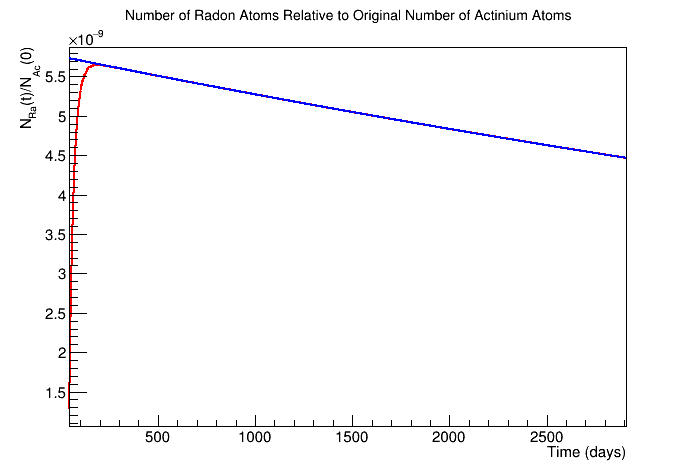
\includegraphics[width=0.8\linewidth]{NRadonvst}
\caption{Comparison of decay equations given in Equations \ref{eq:N3approx1} (red) and \ref{eq:N3approx2} (blue) showing how quickly the approximate solution (blue) becomes valid.}
\end{figure}

\section{Secular Equilibrium}
\label{S:2}
Secular equilibrium occurs between two given isotopes when the decay rates to and from that isotope are equal. This occurs for the decay chain in Eq. \ref{eq:decay_chain} when the decay rate of $^{227}$Ac equals that of $^{219}$Rn which implies that the ratio of concentrations of the two isotopes is approximately constant. We can see from Eq. \ref{eq:N3approx1} that this state is reached when the ratio of the relative concentrations of the isotopes is equal to the ratio of the half-lives of the isotopes. That is, at equilibrium the following relationship holds:
\[
\frac{N_{Rn}(t)}{N_{Ac}(t)}\approx \frac{\lambda_{Ac}}{\lambda_{Rn}}=\frac{t^{(Rn)}_{1/2}}{t^{(Ac)}_{1/2}}\approx5.76\times 10^{-9}.
\]
\begin{figure}[h]
\centering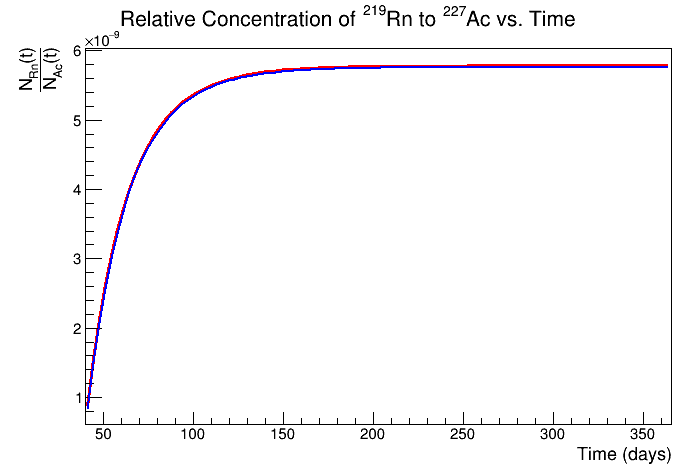
\includegraphics[width=0.8\linewidth]{RelRadonConcentrationvst}
\caption{Relative concentration of $^{219}$Ra to $^{227}$Ac versus time demonstrating that equilibrium is reached after $\sim$180 days. The red curve is the exact solution given by the ratio of Eq. \ref{eq:N3} to Eq. \ref{eq:N0}. The approximate solution (blue) is given by the ratio of Eq. \ref{eq:N3approx1} to Eq. \ref{eq:N0}.}
\end{figure}
Perhaps a simpler way of looking at this is to realize that at equilibrium the decay rate of Ac-227 and Rn-219 must be equal. The decay rate of an isotope as a function of time is given by $\frac{dN(t)}{dt}=-\lambda N_0e^{-\lambda t}$, where $\lambda$ is the lifetime of the isotope and $N_0$ is the number of atoms at $t=0$. Since the decay rates are equal we have
\begin{equation}
\lambda_{Ac}N_0^{(Ac)}e^{-\lambda_{Ac}t}=\lambda_{Rn}N_0^{(Rn)}e^{-\lambda_{Rn}t}\longrightarrow\frac{N_0^{(Ac)}e^{-\lambda_{Ac}t}}{t_{1/2}^{(Ac)}}=\frac{N_0^{(Rn)}e^{-\lambda_{Rn}t}}{t_{1/2}^{(Rn)}}
\end{equation}
For $t<<t$ i.e. the system is in secular equilibrium at $t=0$, we have
\[
\frac{N_0^{(Ac)}}{t_{1/2}^{(Ac)}}=\frac{N_0^{(Rn)}}{t_{1/2}^{(Rn)}}.
\]

\section{Approximate Secular Equilibrium and Equilibrium Constants}
\label{S:3}
\footnote{This derivation follows that of http://www.med.harvard.edu/jpnm/physics/nmltd/radprin/sect2/2.2/2\_2.3.html.}
In the case where the half-life of the parent isotope is much longer than the daughters, secular equilibrium can be approximately reached. However, secular equilibrium is only approximate when considering a set amount of the parent isotope since the activity of each isotope eventually decays away at the half-life of the parent. For decay chains such as Ac-227 with the parent isotope having a longer half-life (by factors of 100-1000) than the daughters a small correction must be applied to the equilibrium value to correctly calculate the activity of the daughters. Intuitively, this can be thought of as coming from the fact that it takes the system (decay chain) a finite amount of time to adjust to the reduced parent activity. Thus, after approximate equilibrium is reached, the activity of the daughters at any given time is greater than that of the parent isotope. The ratio of the daughter activity to that of the parent is called the ``equilibrium constant''. 

To see this first we can define the activity $A_i$ of a given isotope $i$ using Eq \ref{eq:decay_chain} as $A_i(t)=\lambda_iN_i(t)$. For the parent isotope ($i=0$) this becomes
\begin{equation}
\label{eq:p_activity}
A_0(t)=\lambda_0N_0(0)e^{-\lambda_0t}\equiv A_0(0)e^{-\lambda_0t}.
\end{equation}
The activity of the first daughter is likewise given by
\begin{equation}
\label{eq:d1_activity}
A_1(t)=\lambda_0\lambda_1N_0(0)\left(e^{-\lambda_0t}-e^{-\lambda_1t}\right)=A_0(0)\frac{\lambda_1}{\lambda_1-\lambda_0}\left(e^{-\lambda_0t}-e^{-\lambda_1t}\right).
\end{equation}
The equilibrium constant or ratio of the activity of the daughter to the parent is given by 
\begin{equation}
\label{eq:equil_const_1}
k_1=\frac{A_1(t)}{A_0(t)}=\frac{\lambda_1}{\lambda_1-\lambda_0}\left(\frac{e^{-\lambda_0t}-e^{-\lambda_1t}}{e^{-\lambda_0t}}\right)=\frac{\lambda_1}{\lambda_1-\lambda_0}\left(1-e^{-(\lambda_1-\lambda_0)t}\right).
\end{equation}
After several of the (comparatively short) daughter half-lives this goes to 
\begin{equation}
\label{eq:k1}
 k_1\xrightarrow[~]{t>>t_{1/2}^{(1)}}\frac{\lambda_1}{\lambda_1-\lambda_0}=\frac{t_{1/2}^{(0)}}{t_{1/2}^{(0)}-t_{1/2}^{(1)}}
\end{equation}
Likewise for the activity of the second generation we find
\begin{equation}
\label{eq:d1_activity}
A_2(t)=\lambda_0N_0(0)\frac{\lambda_1\lambda_2}{\lambda_1-\lambda_0}\left(\frac{e^{-\lambda_0t}-e^{-\lambda_1t}}{\lambda_2-\lambda_0}-\frac{e^{-\lambda_1t}-e^{-\lambda_2t}}{\lambda_2-\lambda_1}\right)=A_0(0)\frac{\lambda_1\lambda_2}{\lambda_1-\lambda_0}\left(e^{-\lambda_0t}-e^{-\lambda_1t}\right).
\end{equation}
Once again we take the ratio of the activity of the second generation to the parent to find the equilibrium constant.
\begin{equation}
\label{eq:equil_const_2}
k_2=\frac{A_2(t)}{A_0(t)}=\frac{\lambda_1\lambda_2}{\lambda_1-\lambda_0}\left(\frac{e^{-\lambda_0t}-e^{-\lambda_1t}}{\lambda_2-\lambda_0}-\frac{e^{-\lambda_1t}-e^{-\lambda_2t}}{\lambda_2-\lambda_1}\right)\Big/e^{-\lambda_0t}.
\end{equation}
After several daughter half-lives the second term in the parentheses becomes negligble and the first term goes to $1/(\lambda_2-\lambda_0)$ giving
\begin{equation}
\label{eq:k2}
k_2\xrightarrow[~]{t>>t_{1/2}^{(2)}}\frac{\lambda_1}{\lambda_1-\lambda_0}\frac{\lambda_2}{\lambda_2-\lambda_0}=\frac{t_{1/2}^{(0)}}{t_{1/2}^{(0)}-t_{1/2}^{(1)}}=k_1\frac{t_{1/2}^{(0)}}{t_{1/2}^{(0)}-t_{1/2}^{(2)}}.
\end{equation}
In general we can show that $k_i$ is given recursively by
\[
k_i=k_{i-1}\frac{t_{1/2}^{(0)}}{t_{1/2}^{(0)}-t_{1/2}^{(i)}},~~~~~x=1,2...
\]

The net effect of this non-equilibrium correction on the activity of the daughter isotopes in the Ac-227 decay chain is to give a slightly higher decay rate for daughters than for the parent, Ac-227. The non-equilibrium constants for the main decay branches of Ac-227 are calculated in \cite{Kossert2015}. Table 1 in this paper gives a nice summary of the results. I was able to reproduce this table using the probabilities listed and the half-life values from the online interactive IAEA chart of the nuclides. Summing all the alpha decays from this table for each decay of the parent Ac-227 we would expect about 5.015 total alpha decays (parent and daughters included).

%% The Appendices part is started with the command \appendix;
%% appendix sections are then done as normal sections
%% \appendix

%% \section{}
%% \label{}

%% References
%%
%% Following citation commands can be used in the body text:
%% Usage of \cite is as follows:
%%   \cite{key}          ==>>  [#]
%%   \cite[chap. 2]{key} ==>>  [#, chap. 2]
%%   \citet{key}         ==>>  Author [#]

%% References with bibTeX database:

\bibliographystyle{abbrv}
\bibliography{sample.bib}

%% Authors are advised to submit their bibtex database files. They are
%% requested to list a bibtex style file in the manuscript if they do
%% not want to use model1-num-names.bst.

%% References without bibTeX database:

% \begin{thebibliography}{00}

%% \bibitem must have the following form:
%%   \bibitem{key}...
%%

% \bibitem{}

% \end{thebibliography}


\end{document}

%%
